%% !TEX TS-program = xelatex
%% !TEX encoding = UTF-8 Unicode

% Spring 2020 - Summer 2020 - Fall 2020
% Tristan Hill, May 07, 2020 - June 12, 2020 - July 08, 2020
% Module 7 - Frequency Filters
% Topic 1 - What is a Frequency Filter

\documentclass[fleqn]{beamer} % for presentation (has nav buttons at bottom)

\usepackage{/home/thill/Documents/lectures/measurements_lectures/measurements_lectures}


\author{ME3023 - Measurements in Mechanical Systems} % original formatting from Mike Renfro, September 21, 2004

\newcommand{\MNUM}{6\hspace{2mm}} % Module number
\newcommand{\TNUM}{1\hspace{2mm}} % Topic number 
\newcommand{\moduletitle}{Frequency Filters}
\newcommand{\topictitle}{What is a Frequency Filter} 

\newcommand{\sectiontitleI}{Signal, Amplitude, and Frequency}
\newcommand{\sectiontitleII}{Filter Concept}
\newcommand{\sectiontitleIII}{High-Pass, Low-Pass, and Band-Pass}
\newcommand{\sectiontitleIV}{Applications}

% custom box
\newsavebox{\mybox}

\title{Module \MNUM - \moduletitle}

\date{Mechanical Engineering\vspc Tennessee Technological University}

\begin{document}

\lstset{language=MATLAB,basicstyle=\ttfamily\small,showstringspaces=false}

\frame{\titlepage \center\begin{framed}\Large \textbf{Topic \TNUM - \topictitle}\end{framed} \vspace{5mm}}

% Section 0: Outline
\frame{
\large \textbf{Topic \TNUM - \topictitle} \vspace{3mm}\\

\begin{itemize}

	\item \sectiontitleI    \vspc % Section I
	\item \sectiontitleII 	\vspc % Section II
	\item \sectiontitleIII 	\vspc %Section III
	\item \sectiontitleIV 	\vspc %Section IV

\end{itemize}

}

% Section I:
\section{\sectiontitleI}

% Section I - Frame I:
\frame{
\frametitle{\sectiontitleI}

{\R Signal}, {\G Amplitude}, and {\B Frequency}\vspace{2mm}\\
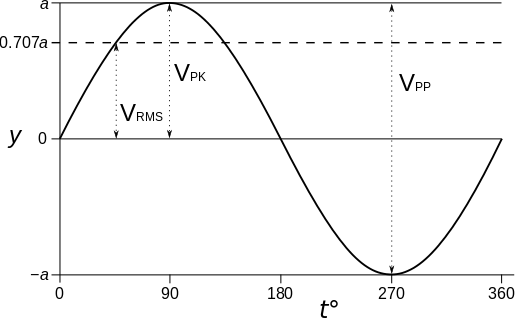
\includegraphics[scale=.25]{amplitude_frequency.png} 
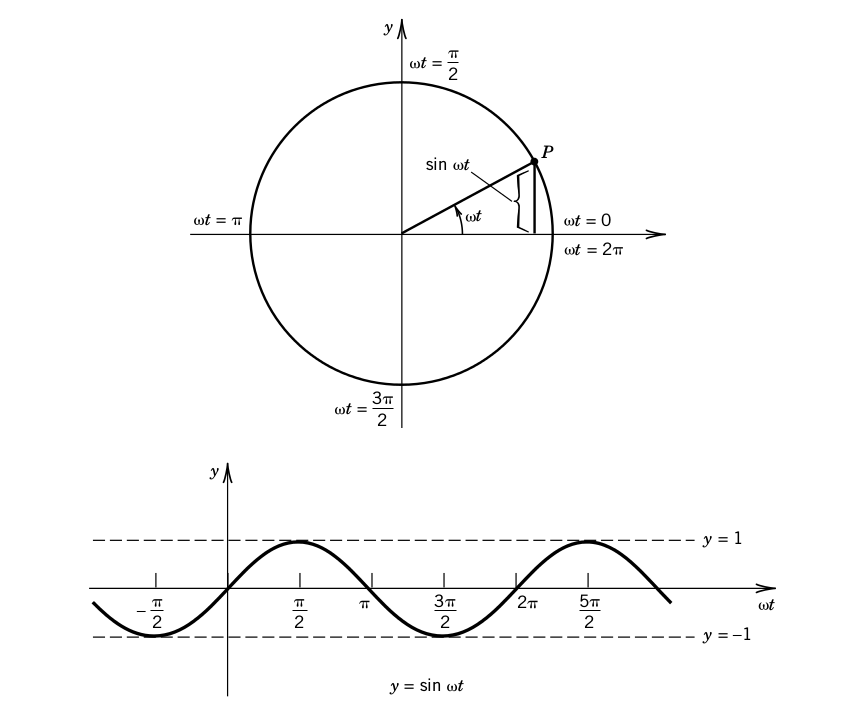
\includegraphics[scale=.25]{unit_circle.png}
					
What is the relationship between the unit circle and frequency?\vspace{5mm}\\


}


% Section I - Frame II:
\frame{ \small
\frametitle{\sectiontitleI}

\begin{multicols}{2}
Signals can be composed of multiple {\it frequency components}. \\ (see Fourier Analysis Ch2).\vspace{3mm}\\

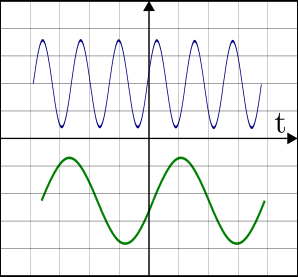
\includegraphics[scale=.4]{signal_addition.png}

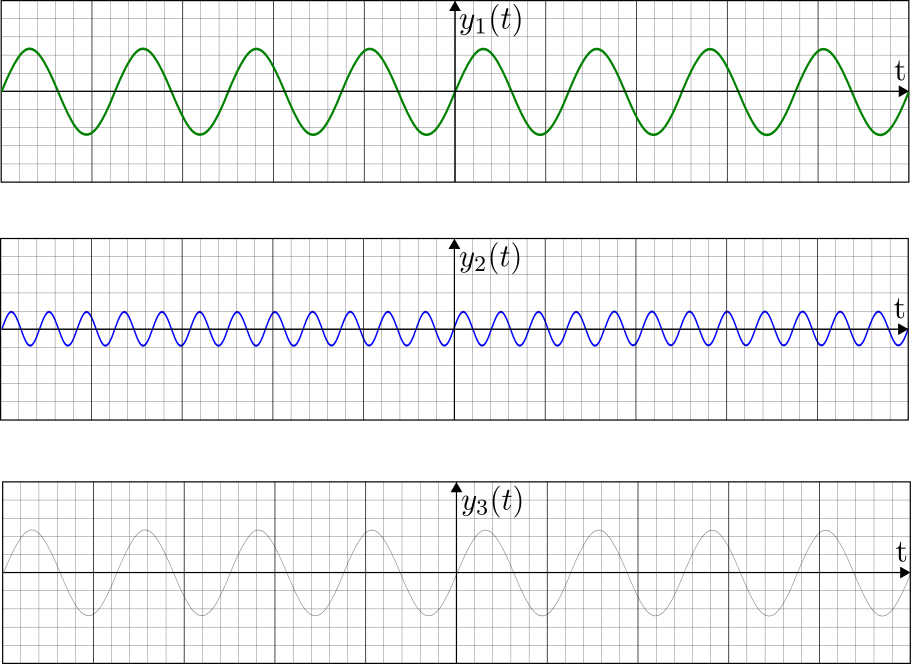
\includegraphics[scale=.30]{frequency_components.png}
\end{multicols}

}

% Section I - Frame III:
\frame{ \small
\frametitle{\sectiontitleI}


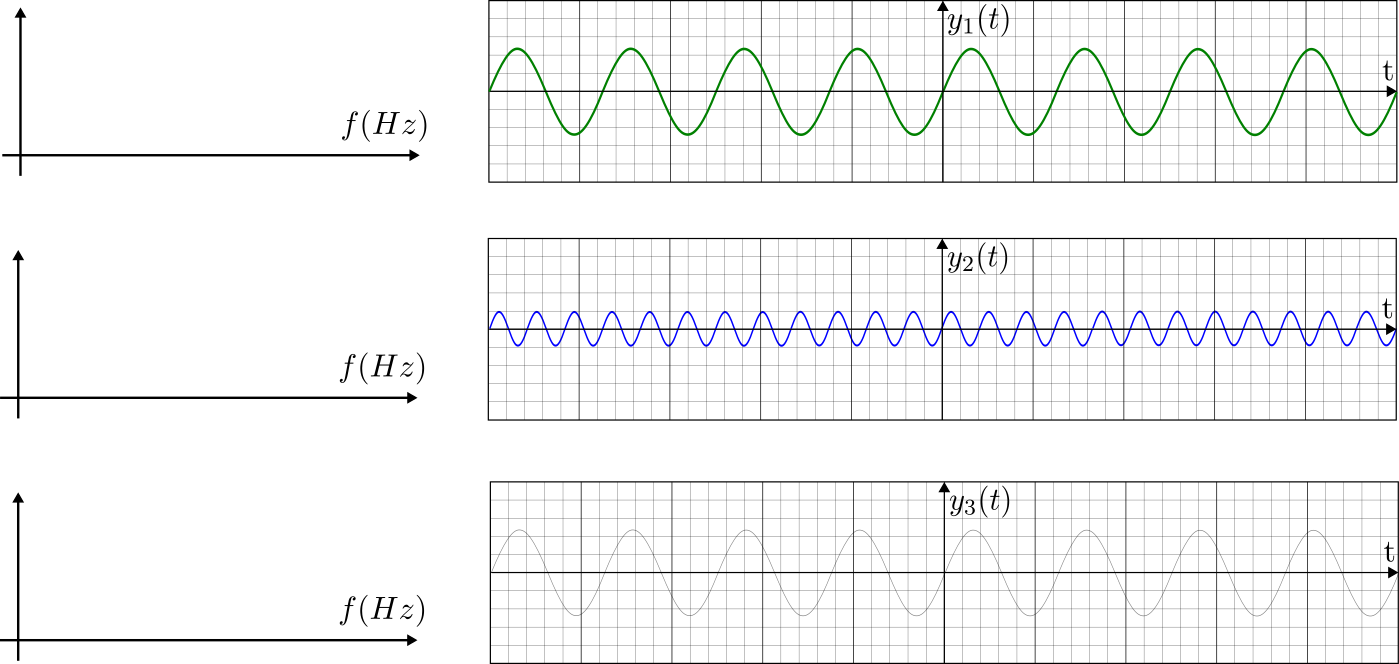
\includegraphics[scale=.35]{frequency_domain.png}

}




% Section II:
\section{\sectiontitleII}

% Section II - Frame I:
\frame{ \small
\frametitle{\sectiontitleII}

A {\PR raw signal} is input to a {\OR frequency filter} and a {\PN filtered signal} is output. \vspace{5mm}

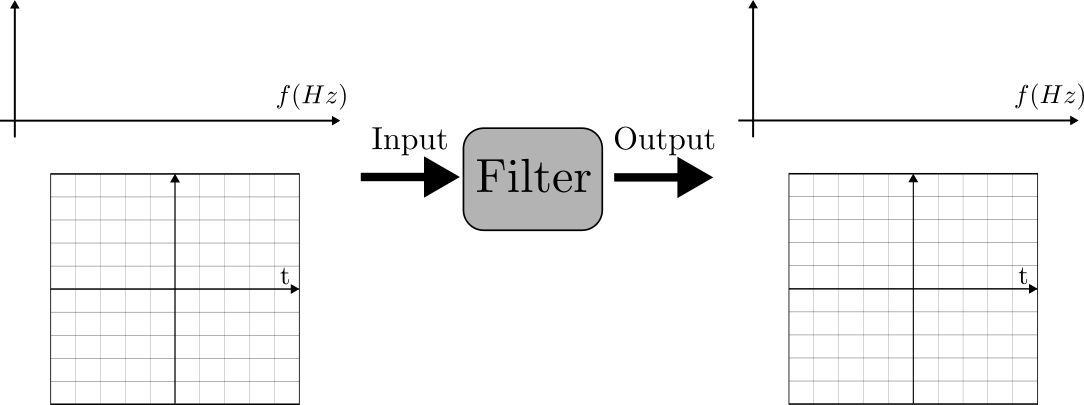
\includegraphics[scale=.45]{filter_concept.png}

} 

% Section II - Frame II:
\frame{
\frametitle{\sectiontitleII}

So what is inside the {\it grey box}? \vspace{10mm} \\

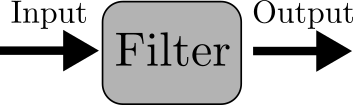
\includegraphics[scale=.5]{grey_box.png} \vspace{5mm} \\
How does it work? 

}


% Section II - Frame II:
\frame{
\frametitle{\sectiontitleII }

Filters are constructed from time-varying circuits. The most basic of which is the {\B RC filter}.
\begin{multicols}{2}

First Order Model
\[ \tau \dot{y}+y=KA \sin(\omega t) \]

Response Equation
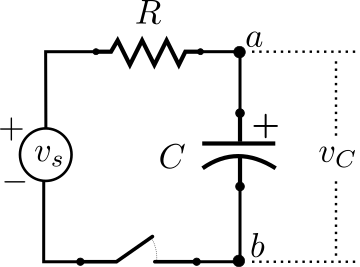
\includegraphics[scale=.5]{rc_circuit.png} \vspace{5mm} \\
\end{multicols}

\[ y(t)=Ce^{-\frac{t}{\tau}}+\frac{KA}{\sqrt{1+(\omega\tau)^2}}\sin(\omega t-\tan^{-1}(\omega\tau)) \]

}


% Section III:
\section{\sectiontitleIII}

% Section III - Frame I:
\frame{\small
\frametitle{\sectiontitleIII}
	
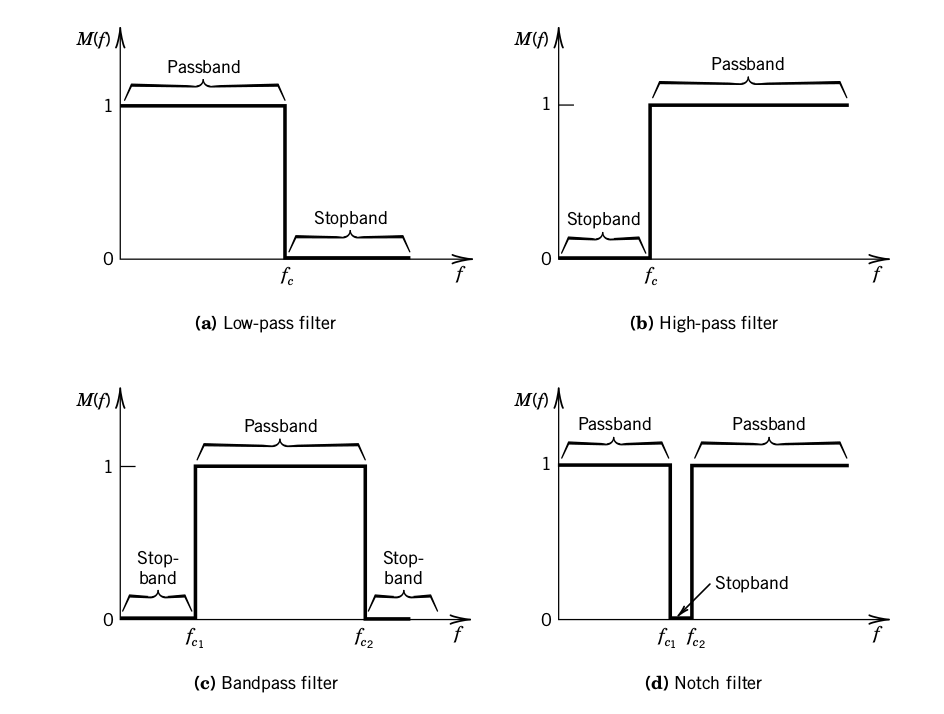
\includegraphics[scale=.25]{filter_types.png} \vspace{5mm} \\

}

% Section III - Frame II:
\frame{\small
\frametitle{\sectiontitleIII}
Physical frequency filters do not behave in an ideal manner as the previous figure shows. The filter characteristics are frequency dependent. 

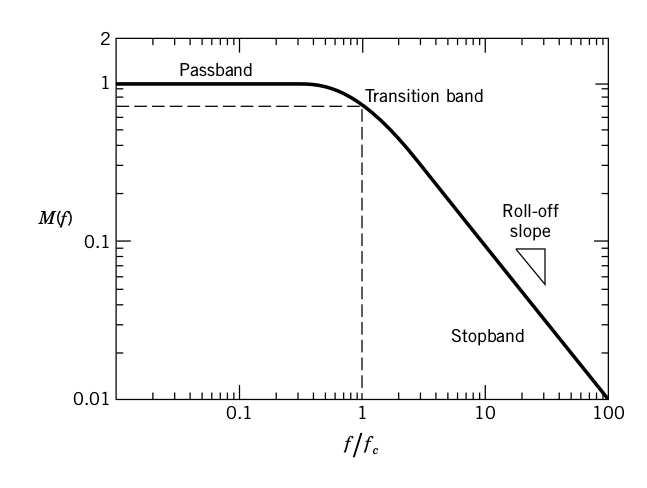
\includegraphics[scale=.3]{bode_diagram.png} \vspace{5mm} \\

	
	
}

%% Section IV:
\section{\sectiontitleIV}

% Section IV - Frame I:
\frame{\small
\frametitle{\sectiontitleIV}

	
	Finally, what are filters used for? 
	\begin{itemize}
		\item 
		\item 
		\item	
	\end{itemize}

}
	
\end{document}



